\section{Results and Discussion}

\subsection{Temperature Distribution}

Figure~\ref{fig:contours} compares the numerical temperature distribution obtained using the Point Gauss-Seidel solver with the analytical solution of the Laplace equation. The two temperature fields exhibit close agreement throughout the computational domain. The similarity between the numerical and analytical contours supports the correctness of the governing equation, spatial discretization, and boundary-condition implementation.

\begin{figure}[H]
    \centering
    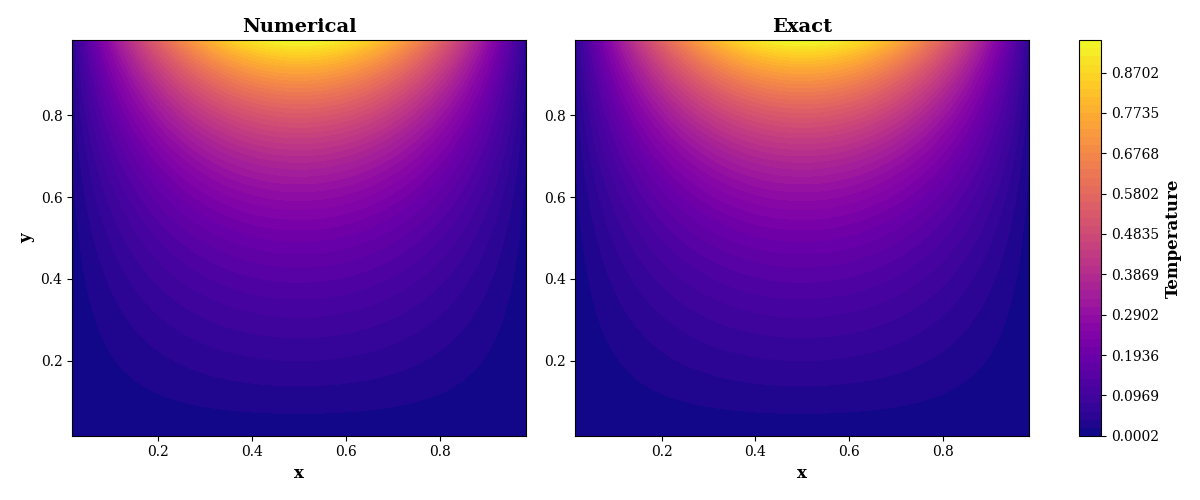
\includegraphics[width=\textwidth]{figures/temperature_contours.png}
    \caption{Comparison of the numerical and analytical temperature distributions obtained using the Point Gauss-Seidel solver.}
    \label{fig:contours}
\end{figure}

%%%%%%%%%%%%%%%%%%%%%%%%%%%%%%%%%%%%%%%%%%%%%%%%%%%%%%%%%%%%%

\subsection{Error Field}

The pointwise difference between the numerical and analytical temperature distributions provides a quantitative assessment of the numerical error. Figure~\ref{fig:error} shows the spatial distribution of this difference.

The error field illustrates the local discrepancies between the computed and analytical solutions. A quantitative assessment of the spatial accuracy can additionally be obtained by evaluating error norms and examining their variation across different mesh resolutions.

\begin{figure}[H]
    \centering
    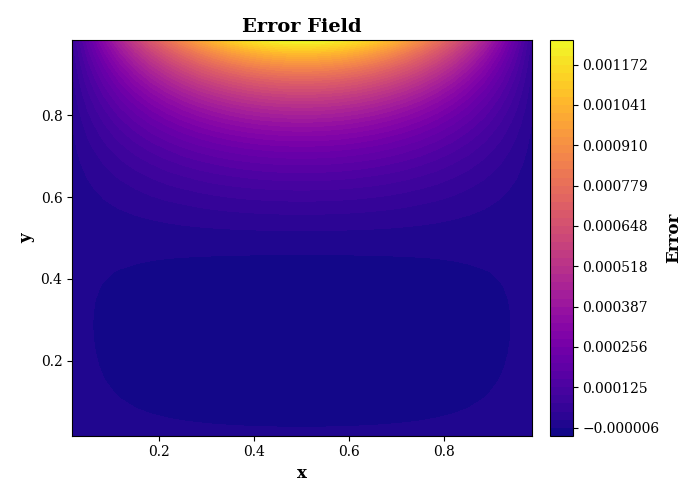
\includegraphics[width=0.65\textwidth]{figures/error_field.png}
    \caption{Spatial distribution of the error between the numerical and analytical temperature fields obtained using Point Gauss-Seidel.}
    \label{fig:error}
\end{figure}

%%%%%%%%%%%%%%%%%%%%%%%%%%%%%%%%%%%%%%%%%%%%%%%%%%%%%%%%%%%%%

\subsection{Convergence History}

The convergence behavior of the Point Gauss-Seidel solver was monitored using the $L_2$ residual norm. Figure~\ref{fig:residual} presents the residual history as a function of both iteration number and CPU time.

The residual decreases toward the prescribed tolerance, indicating convergence toward the solution of the discretized governing equation. The residual-time history also provides a baseline for evaluating the computational performance of the accelerated iterative methods considered in the following subsections.

\begin{figure}[H]
    \centering
    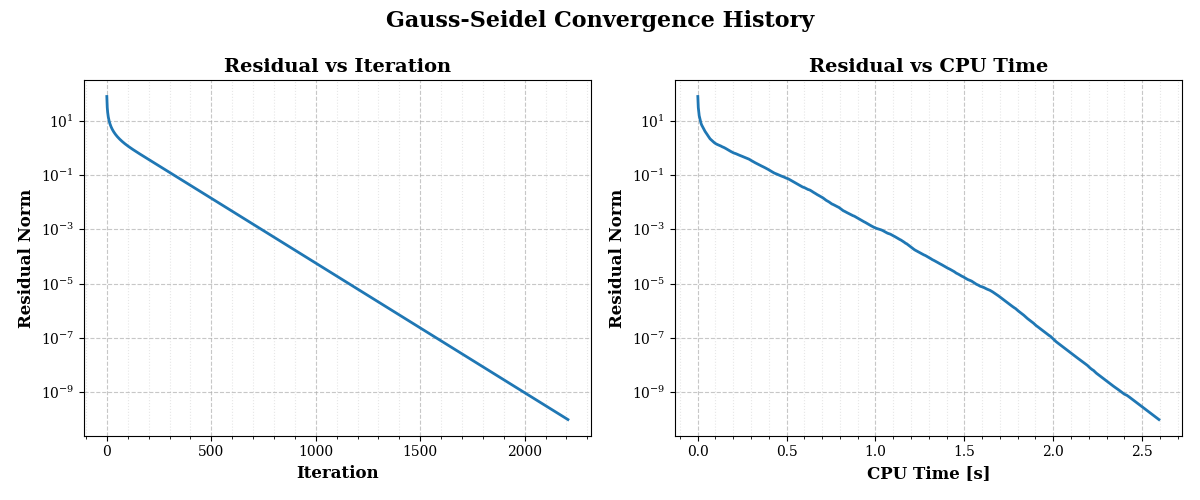
\includegraphics[width=\textwidth]{figures/residual_history.png}
    \caption{Residual convergence histories of the Point Gauss-Seidel solver as functions of iteration count and CPU time.}
    \label{fig:residual}
\end{figure}

%%%%%%%%%%%%%%%%%%%%%%%%%%%%%%%%%%%%%%%%%%%%%%%%%%%%%%%%%%%%%

\subsection{Line-Cut Comparison}

To further assess the numerical solution, horizontal and vertical temperature profiles were extracted at selected locations within the computational domain and compared with the corresponding analytical profiles.

As shown in Figure~\ref{fig:linecuts}, the numerical and analytical temperature profiles exhibit close agreement along the selected cuts. This comparison provides an additional assessment of the spatial variation of the computed temperature field.

\begin{figure}[H]
    \centering
    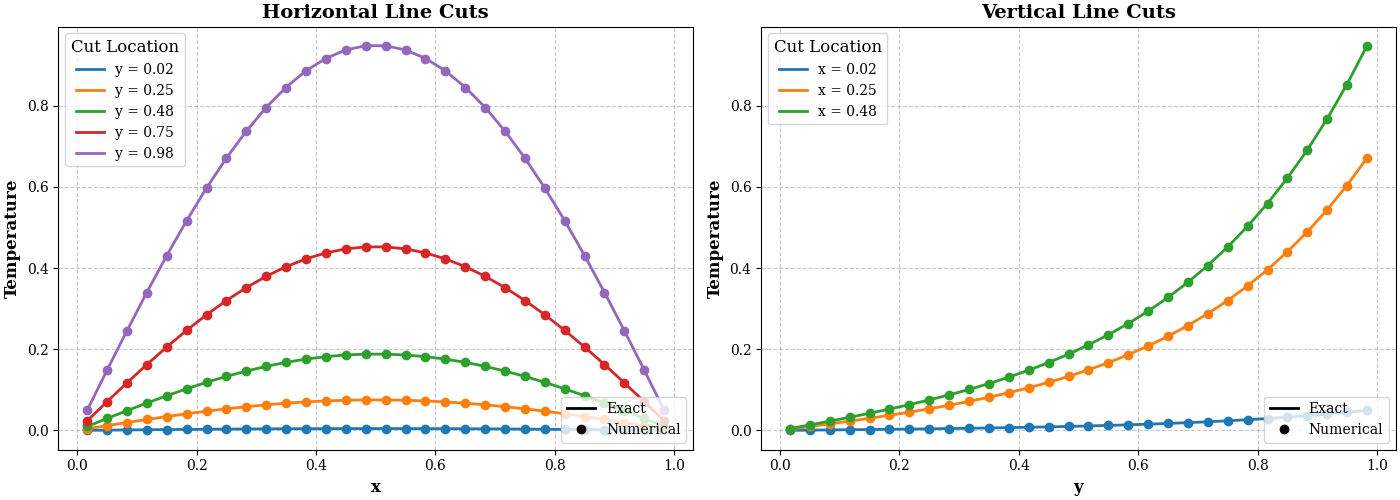
\includegraphics[width=\textwidth]{figures/line_cuts.png}
    \caption{Comparison of numerical and analytical temperature profiles along selected horizontal and vertical line cuts.}
    \label{fig:linecuts}
\end{figure}

%%%%%%%%%%%%%%%%%%%%%%%%%%%%%%%%%%%%%%%%%%%%%%%%%%%%%%%%%%%%%

\subsection{SOR Convergence and Computational Cost}

The effect of the relaxation factor on convergence was investigated using the Successive Over-Relaxation (SOR) method. The Point Gauss-Seidel solver and SOR with relaxation factors $\omega=1.1$, $1.3$, and $1.5$ were evaluated on a $40\times40$ mesh with a residual tolerance of $10^{-12}$.

Figure~\ref{fig:gs_sor_convergence} compares the residual histories as functions of iteration number and CPU time. Increasing the relaxation factor from $1.1$ to $1.5$ reduces the iteration count from 3823 to 1549. In the recorded runs, SOR with $\omega=1.3$ and $1.5$ also requires less CPU time than the Point Gauss-Seidel solver. However, the results for $\omega=1.1$ show that reducing the iteration count does not necessarily reduce the total computation time.

The corresponding iteration counts, CPU times, and final residuals are reported in Table~\ref{tab:gs_sor_comparison}.

\begin{figure}[H]
    \centering
    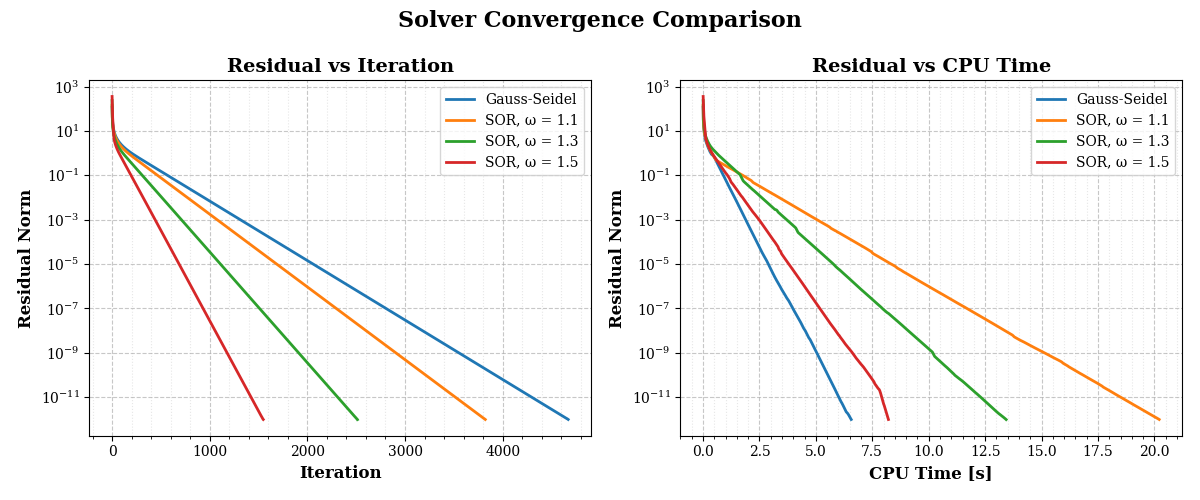
\includegraphics[width=\textwidth]{figures/gs_sor_convergence.png}
    \caption{Residual convergence histories of Point Gauss-Seidel and SOR with different relaxation factors on a $40\times40$ mesh. The panels show residual versus iteration count and residual versus CPU time.}
    \label{fig:gs_sor_convergence}
\end{figure}

\begin{table}[H]
    \centering
    \small
    \caption{Convergence and computational performance of Point Gauss-Seidel and SOR on a $40\times40$ mesh.}
    \label{tab:gs_sor_comparison}
    \begin{tabular}{lrrrr}
        \toprule
        \textbf{Solver} &
        \textbf{$\omega$} &
        \textbf{Iterations} &
        \textbf{CPU Time [s]} &
        \textbf{Final Residual} \\
        \midrule
        Gauss-Seidel & --  & 4672 & 6.1124 & $9.94\times10^{-13}$ \\
        SOR          & 1.1 & 3823 & 7.7521 & $9.93\times10^{-13}$ \\
        SOR          & 1.3 & 2514 & 5.4302 & $9.84\times10^{-13}$ \\
        SOR          & 1.5 & 1549 & 3.2679 & $9.92\times10^{-13}$ \\
        \bottomrule
    \end{tabular}
\end{table}

%%%%%%%%%%%%%%%%%%%%%%%%%%%%%%%%%%%%%%%%%%%%%%%%%%%%%%%%%%%%%

\subsection{Line-SOR Convergence and Computational Cost}

The Line-SOR method was compared with point-wise SOR using $\omega=1.1$ on a $40\times40$ mesh and with the same residual tolerance of $10^{-12}$.

Figure~\ref{fig:line_sor_convergence} presents the residual histories of the two methods as functions of iteration number and CPU time. Line-SOR requires 1909 iterations, compared with 3823 iterations for point-wise SOR. The corresponding CPU times are 2.2451 s and 8.0495 s, respectively. In this benchmark, Line-SOR therefore achieves convergence in approximately half as many iterations and reduces the recorded CPU time by approximately 72\%.

The comparison is summarized in Table~\ref{tab:line_sor_comparison}. These results illustrate the benefit of solving for temperature corrections along an entire line rather than updating each control volume independently.

\begin{figure}[H]
    \centering
    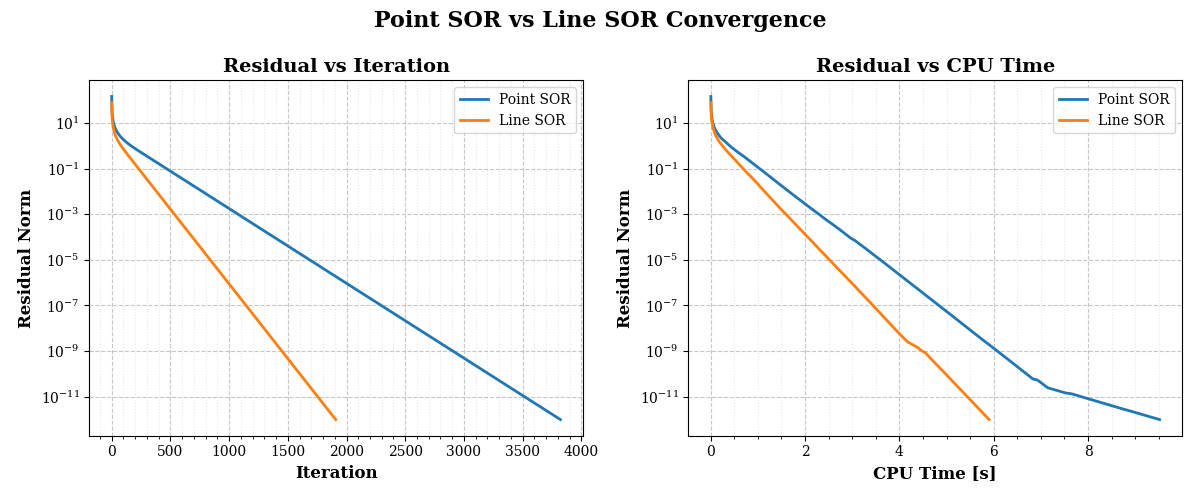
\includegraphics[width=\textwidth]{figures/point_line_sor_convergence.png}
    \caption{Residual convergence histories of Point-SOR and Line-SOR with $\omega=1.1$ on a $40\times40$ mesh. The panels show residual versus iteration count and residual versus CPU time.}
    \label{fig:line_sor_convergence}
\end{figure}

\begin{table}[H]
    \centering
    \small
    \caption{Convergence and computational performance of Point-SOR and Line-SOR with $\omega=1.1$ on a $40\times40$ mesh.}
    \label{tab:line_sor_comparison}
    \begin{tabular}{lrrrr}
        \toprule
        \textbf{Solver} &
        \textbf{$\omega$} &
        \textbf{Iterations} &
        \textbf{CPU Time [s]} &
        \textbf{Final Residual} \\
        \midrule
        Point SOR & 1.1 & 3823 & 8.0495 & $9.93\times10^{-13}$ \\
        Line SOR  & 1.1 & 1909 & 2.2451 & $1.00\times10^{-12}$ \\
        \bottomrule
    \end{tabular}
\end{table}

%%%%%%%%%%%%%%%%%%%%%%%%%%%%%%%%%%%%%%%%%%%%%%%%%%%%%%%%%%%%%

\subsection{Fully Implicit Direct Solver}

The fully implicit direct method assembles the discretized equations into a single linear system and solves for the complete temperature field. Unlike the iterative methods, it does not require repeated temperature updates to reach a prescribed residual tolerance.

\subsubsection{CPU-Time Comparison Across Mesh Sizes}

The computational performance of SOR, Line-SOR, and the fully implicit direct method was evaluated for mesh sizes $N=10$, $20$, $30$, and $40$. The iterative methods were tested using relaxation factors $\omega=1.3$ and $1.5$, while the direct method was evaluated on each mesh without an iterative relaxation factor.

Figure~\ref{fig:solver_cpu_time_comparison} compares the CPU times of these methods as the mesh is refined. The corresponding iteration counts, CPU times, and final residuals are reported in Table~\ref{tab:solver_cpu_time_comparison}.

For the tested meshes, Line-SOR requires less CPU time than point-wise SOR at the same relaxation factor. The direct method has the lowest recorded CPU time for each of the four mesh sizes. However, the direct solver uses a dense coefficient matrix, and its memory requirements and computational cost are expected to increase rapidly for larger systems. These observations should therefore be interpreted within the tested mesh range.

CPU times were recorded in separate benchmark runs. Small differences between tables for the same mesh and relaxation factor can therefore arise from run-to-run timing variation. Comparisons are best interpreted within each benchmark.

\begin{figure}[H]
    \centering
    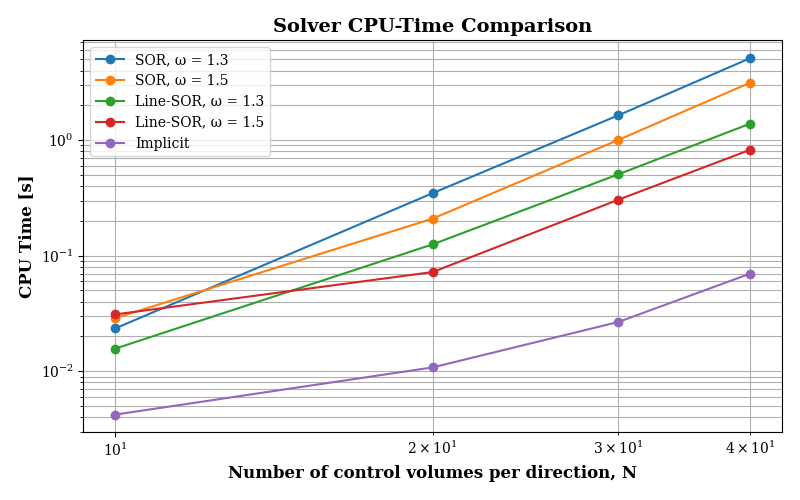
\includegraphics[width=0.9\textwidth]{figures/solver_cpu_time_comparison.png}
    \caption{CPU time versus mesh size for SOR, Line-SOR, and the fully implicit direct solver. The iterative methods are shown for $\omega=1.3$ and $1.5$.}
    \label{fig:solver_cpu_time_comparison}
\end{figure}

\begin{table}[H]
    \centering
    \footnotesize
    \setlength{\tabcolsep}{4pt}
    \caption{Iteration counts, CPU times, and final residuals for SOR, Line-SOR, and the fully implicit direct method at different mesh sizes.}
    \label{tab:solver_cpu_time_comparison}
        \begin{tabular}{rlrrrr}
            \toprule
            \textbf{$N$} &
            \textbf{Solver} &
            \textbf{$\omega$} &
            \textbf{Iterations} &
            \textbf{CPU Time [s]} &
            \textbf{Final Residual} \\
            \midrule
            10 & SOR      & 1.3 & 146    & 0.0248 & $9.86\times10^{-13}$ \\
            10 & SOR      & 1.5 & 174    & 0.0319 & $8.74\times10^{-13}$ \\
            10 & Line-SOR & 1.3 & 68     & 0.0140 & $9.63\times10^{-13}$ \\
            10 & Line-SOR & 1.5 & 135    & 0.0274 & $8.44\times10^{-13}$ \\
            10 & Implicit & --  & Direct & 0.0044 & $2.13\times10^{-14}$ \\
            \midrule
            20 & SOR      & 1.3 & 622    & 0.3904 & $9.63\times10^{-13}$ \\
            20 & SOR      & 1.5 & 374    & 0.2044 & $9.47\times10^{-13}$ \\
            20 & Line-SOR & 1.3 & 307    & 0.1316 & $9.20\times10^{-13}$ \\
            20 & Line-SOR & 1.5 & 176    & 0.0735 & $9.04\times10^{-13}$ \\
            20 & Implicit & --  & Direct & 0.0162 & $7.47\times10^{-14}$ \\
            \midrule
            30 & SOR      & 1.3 & 1410   & 1.6450 & $9.92\times10^{-13}$ \\
            30 & SOR      & 1.5 & 864    & 1.0472 & $9.70\times10^{-13}$ \\
            30 & Line-SOR & 1.3 & 700    & 0.5520 & $9.71\times10^{-13}$ \\
            30 & Line-SOR & 1.5 & 421    & 0.3309 & $9.61\times10^{-13}$ \\
            30 & Implicit & --  & Direct & 0.0433 & $1.73\times10^{-13}$ \\
            \midrule
            40 & SOR      & 1.3 & 2514   & 5.2015 & $9.84\times10^{-13}$ \\
            40 & SOR      & 1.5 & 1549   & 3.1708 & $9.92\times10^{-13}$ \\
            40 & Line-SOR & 1.3 & 1250   & 1.3868 & $9.92\times10^{-13}$ \\
            40 & Line-SOR & 1.5 & 762    & 0.8401 & $9.87\times10^{-13}$ \\
            40 & Implicit & --  & Direct & 0.0976 & $3.50\times10^{-13}$ \\
            \bottomrule
        \end{tabular}%
    
\end{table}

\subsubsection{Verification Against the Analytical Solution}

The fully implicit solution on the $40\times40$ mesh was compared with the analytical temperature field. Figure~\ref{fig:implicit_contours} shows the numerical and analytical temperature distributions side by side, while Figure~\ref{fig:implicit_error} presents the spatial distribution of their difference.

For this mesh, the computed $L_2$ error is $1.6122\times10^{-4}$, and the maximum absolute error is $7.2049\times10^{-4}$. These values quantify the difference between the numerical and analytical solutions. The error reflects the spatial discretization and should be distinguished from the residual, which measures how closely the numerical field satisfies the discrete equations.

\begin{figure}[H]
    \centering
    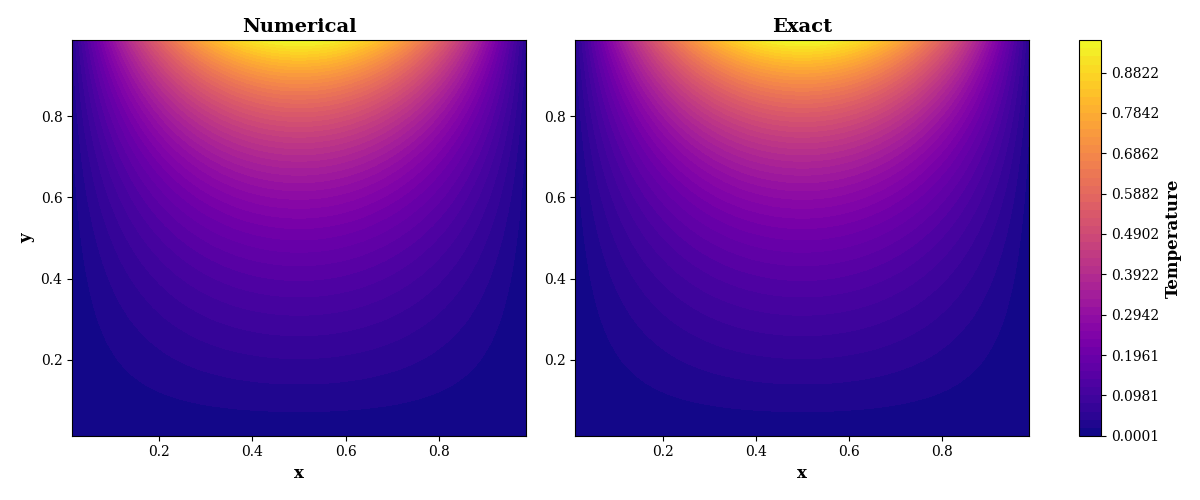
\includegraphics[width=\textwidth]{figures/implicit_temperature_contours.png}
    \caption{Comparison of the fully implicit numerical temperature distribution and the analytical solution on a $40\times40$ mesh.}
    \label{fig:implicit_contours}
\end{figure}

\begin{figure}[H]
    \centering
    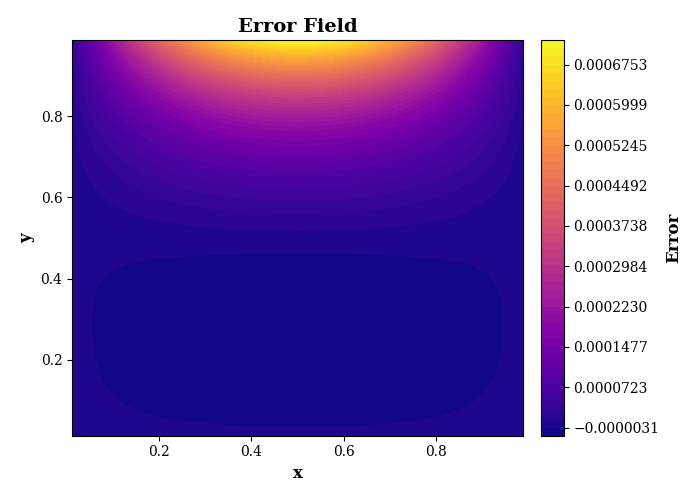
\includegraphics[width=0.7\textwidth]{figures/implicit_error_field.png}
    \caption{Spatial distribution of the temperature error, defined as the fully implicit numerical solution minus the analytical solution, on a $40\times40$ mesh.}
    \label{fig:implicit_error}
\end{figure}